% Simpelt tre
\begin{figure}[H]
    \centering
    \Tree [.null
            [.C:11
                [.F:10
                    [.G:8
                        [.H:6 
                            [.A:3 
                                [.B:1 ]]
                            [.B:1 ] ]
                        [.A:1 ]
                        [.B:1 ] ]
                    [.H:1 
                        [.A:1 
                            [.B:1 ]]]
                    [.B:1 ] ]
                [.G:1 
                    [.A:1 
                        [.B:1 ]]]
            ]
            [.F:1 
                [.G:1
                    [.H:1 ]
                ]
            ]
         ]
    \caption{FP-growth tree}
    \label{fig:fp-tree}
\end{figure}


% Pen greie
\[
\begin{blockarray}{ccccccccccc}
 & f_i,_1 & f_i,_2 & f_i,_3 & f_i,_4 & f_i,_5 & f_i,_6 & f_i,_7 & f_i,_8 & f_i,_9 & f_i,_{10} \\
\begin{block}{c(cccccccccc)}
  Autumn & 1 & 1 & 1 & 3 & 0 & 0 & 1 & 1 & 0 & 1 \\
  Spring & 2 & 1 & 0 & 2 & 0 & 2 & 1 & 2 & 2 & 1 \\
  Winter & 1 & 0 & 2 & 2 & 1 & 0 & 1 & 0 & 1 & 2 \\
\end{block}
\label{matrix: raw-frequency}
\end{blockarray}
 \]
 
 
% Selvtegnede grafer
 
 \begin{center}
    %Non-interpolated Graph
    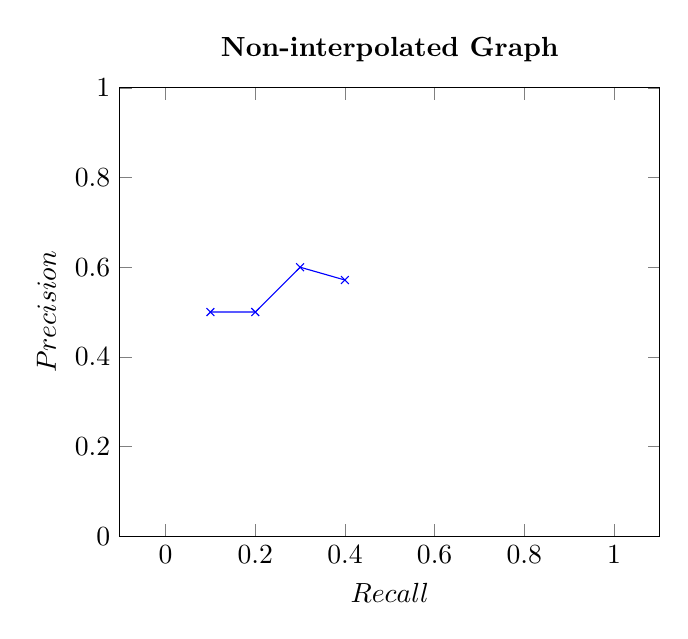
\begin{tikzpicture}
    \begin{axis}[axis equal, title={\textbf{Non-interpolated Graph}},
    % Endrer min max område på aksene
    xmin=0, xmax=1,
    ymin=0, ymax=1,
    xlabel={$\text{Recall} $},
    ylabel={$\text{Precision}$}]
    \addplot+[mark=x] plot coordinates
    { (0.1 , 0.5 ) (0.2 , 0.5) (0.3 , 0.6) (0.4 , 0.5714) };
    \end{axis}
    \end{tikzpicture}
\end{center}
    
    
\begin{center}
    % Interpolated Graph
    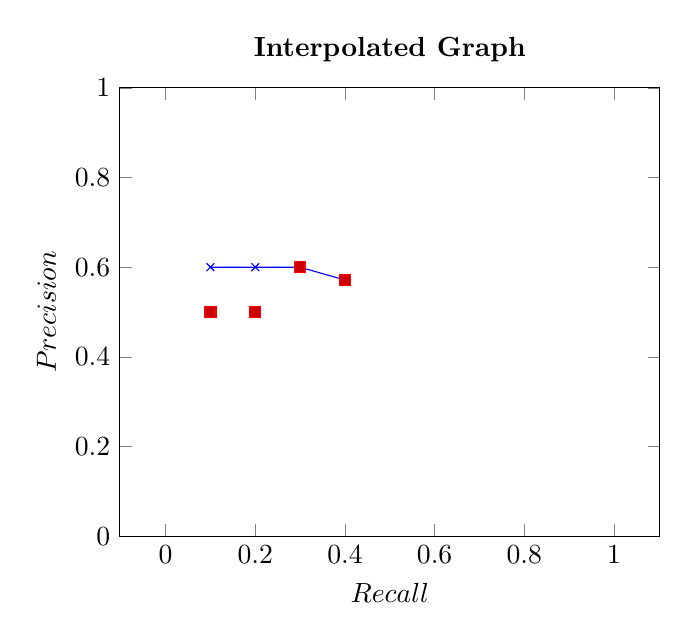
\begin{tikzpicture}
    \begin{axis}[axis equal, title={\textbf{Interpolated Graph}},
    % Endrer min max området på x og y akse
    xmin=0, xmax=1,
    ymin=0, ymax=1,
    xlabel={$\text{Recall} $},
    ylabel={$\text{Precision}$}]
    
    \addplot+[mark=x] plot coordinates
    {(0.1 , 0.6 ) (0.2 , 0.6) (0.3 , 0.6) (0.4 , 0.5714)};
    \addplot+[only marks] coordinates 
    {(0.1 , 0.5 ) (0.2 , 0.5) (0.3 , 0.6) (0.4 , 0.5714)};
    
    \end{axis}
    \end{tikzpicture}\\
    \caption{The blue graph is the interpolated graph of the values in subsection 3.2\\
    The red dots show the points for the non-interpolated graph of the same values}
\end{center}


% VELDIG BREDE TRÆR

\begin{tikzpicture}[scale=0.8]
\centering
\Tree [.S
        What/WP
        happened/VBD
        to/TO
        the/DT
        [.CHUNK\_NNP Tesla/NNP ]
        that/WDT
        [.CHUNK\_NNP Elon/NNP Musk/NNP ]
        shot/NN
        into/IN
        space/NN
        ?/. ]
\end{tikzpicture}

\begin{tikzpicture}[scale=0.5]
\centering
\Tree [.S
        There/EX
        were/VBD
        plenty/NN
        of/IN
        [.CHUNK\_DTJJNNS spectacular/JJ moments/NNS ]
        during/IN
        the/DT
        maiden/JJ
        launch/NN
        of/IN
        [.CHUNK\_NNP SpaceX/NNP ]
        's/POS
        [.CHUNK\_NNP Falcon/NNP Heavy/NNP ]
        rocket/NN
        on/IN
        [.CHUNK\_NNP Tuesday/NNP ]
        ./. ]
\end{tikzpicture}

\begin{tikzpicture}[scale=0.3]
\centering
\Tree [.S
        But/CC
        perhaps/RB
        the/DT
        most/RBS
        dramatic/JJ
        scene/NN
        occurred/VBD
        about/IN
        four/CD
        minutes/NNS
        after/IN
        liftoff/NN
        :/:
        The/DT
        second/JJ
        stage/NN
        of/IN
        the/DT
        rocket/NN
        ,/,
        headed/VBN
        deeper/NN
        into/IN
        space/NN
        ,/,
        discarded/VBD
        the/DT
        white/JJ
        nose/JJ
        cone/NN
        at/IN
        its/PRP\$
        tip/NN
        ./. ]
\end{tikzpicture}

\begin{tikzpicture}[scale=0.8]
\centering
\Tree [.S
        It/PRP
        revealed/VBD
        [.CHUNK\_NNP SpaceX/NNP CEO/NNP Elon/NNP Musk/NNP ]
        's/POS
        cherry/NN
        [.CHUNK\_DTJJNNS red/JJ sports/NNS ]
        car/NN
        ./. ]
\end{tikzpicture}

\begin{tikzpicture}[scale=0.8]
\centering
\Tree [.S
        Behind/IN
        the/DT
        wheel/NN
        was/VBD
        a/DT
        spacesuit-clad/JJ
        mannequin/NN
        ,/,
        named/VBN
        [.CHUNK\_NNP Starman/NNP ]
        ./. ]
\end{tikzpicture}



% MATRISER

\begin{align*}
    \textrm{color}_1 &= 0.5 \begin{bmatrix}
        0 \\
        0 \\
        1 \\
    \end{bmatrix} + \begin{bmatrix}
        0.3 \\
        0.5 \\
        0.8 \\
    \end{bmatrix} = \begin{bmatrix}
        0.15 \\
        0.25 \\
        0.9 \\
    \end{bmatrix}
\end{align*}

\begin{align*}
    \textrm{color}_2 &= 0.5 \begin{bmatrix}
        1 \\
        0 \\
        0 \\
    \end{bmatrix} + \begin{bmatrix}
        0.15 \\
        0.25 \\
        0.9 \\
    \end{bmatrix} = \begin{bmatrix}
        0.575 \\
        0.125 \\
        0.45 \\
    \end{bmatrix}
\end{align*}

\begin{align*}
    \textrm{color}_3 &= 0.5 \begin{bmatrix}
        0 \\
        1 \\
        0 \\
    \end{bmatrix} + \begin{bmatrix}
        0.575 \\
        0.125 \\
        0.45 \\
    \end{bmatrix} = \begin{bmatrix}
        0.286 \\
        0.5625 \\
        0.225 \\ 
    \end{bmatrix}
\end{align*}